\subsection{The Definition of a Vector Space}

{\large \textbf{Lecture 1}}

Before we formally define a vector space, let's introduce some examples of vector spaces.

\begin{example}[\textbf{Vector Spaces}]
    \phantom{}
    \begin{enumerate}
        \item $V = \R^2.$ We have $\vx + \vy = \cv{x_1 \\ x_2} + \cv{y_1 \\ y_2} = \cv{x_1+y_1 \\ x_2+y_2}$ and $c\vx = c\cv{x_1 \\ x_2} = \cv{cx_1 \\ cx_2}.$
        \item $V =  \mP_n(\R) = \{ a_0 + a_1x + \cdots + a_nx^n : a_i \in \R \} =$ polynomiasl of degree $\leq n$ with coefficients in $\R$.  \\
        We can add: $(a_0 + \cdots + a_nx^n) + (b_0 + \cdots + b_nx^n) = (a_0 + b_0) + \cdots + (a_n + b_n)x^n.$    \\
        We can scale: $c(a_0 + a_1 + \cdots + a_nx^n) = (ca_0)+ (ca_1)x + \cdots + (ca_n)x^n$.
        \item $V = M_{m \times n}{(\R)} = \left\{
           \begin{bmatrix}
            &  & \\ 
            & a_{ij} & \\ 
            &  & 
           \end{bmatrix}: a_{ij} \in \F\right\}.$   \\
           Add: $\cv{a_{ij}} + \cv{b_{ij}} = \cv{a_{ij} + b_{ij}}$ \qquad AND \qquad Scale: $c\cv{a_{ij}} =  \cv{ca_{ij}}$. \\
           \phantom{}\\
           \textbf{Oberservation:} $\R^4 \text{ vs. } \mP_3(\R) \text{ vs. } M_{2 \times 2}{(\R)}.$ These are essentially the same. This is an example of an isomorphism (identical form).
           In general, $\R^{mn} \cong \mP_{mn - 1}(\R) \cong M_{m \times n}{(\R)}.$ 
        \item $V = \{\text{functions } f: \R \to \R\}, f,g \in V$. We can add them to get $(f + g)(x) + f(x) + g(x)$ and we can scale by $c \in \R$
              to get $(cf)(x) = c(f(x)).$
        \item $C = \left\{f: \R \to \R: f \text{ is continuous}\right\}$. If $f, g \in V$, then $f + g \in V.$ If $c \in \R, f \in V$, then $cf \in V$. This is a subspace of $V$.
        \item $D = \left\{  f: \R \to \R: f \text{ is infinitely differentiable} \right\}$ is also a subspace of $V$.
    \end{enumerate} 
\end{example}

\begin{note}
    The vector spaces in example 5 and example 6 are \textbf{isomorphic}. But example 4 and 6 \& example 5 and 6 are both not.
\end{note}

\begin{definition}[\textbf{Vector Space}]
    A vector space over $\F$ is a set $V$ together with $+: V \times V \to V$ (vector addition)
    so that $\forall \vx, \vy \in V$, $\vx + \vy \in V$ and an operation $\cdot : \F \times V \to V$ (scalar multiplication)
    so that $\forall c \in \F$ and $\vx \in V$, $c \cdot \vx \in V$. \\

    These operations must satisfy the following \textbf{vector space axioms}:
    \begin{enumerate}
        \item $\forall \vx, \vy \in V, \vx + \vy = \vy + \vx$.
        \item $\forall \vx, \vy, \vz \in V$, $(\vx + \vy) + \vz = \vx + (\vy + \vz)$.
        \item $\forall \vx, \vy \in V$ and $c \in \F, c \cdot (\vx + \vy) = c \cdot \vx + c \cdot \vy.$
        \item $\forall \vx \in V$ and $c, d \in \F, (c + d) \cdot \vx = c \cdot \vx + d \cdot \vx.$
        \item $\forall \vx \in V$ and $c, d \in \F, (cd) \cdot \vx = c \cdot (d \cdot \vx).$
        \item $\forall \vx \in V, 1 \cdot \vx = \vx.$
        \item $\exists \vzero \in V \st \forall \vx \in V, \vzero + \vx = \vx + \vzero = \vx$.
        \item $\forall \vx \in V, \exists (-\vx) \in V \st \vx + (-\vx) =  (-\vx) + \vx = \vzero.$
    \end{enumerate}
\end{definition}

\begin{remark}
    \phantom{}
    \begin{enumerate}
        \item There is a unique $\vzero$ as in axiom 7.
        \item $\forall \vx$, there is a unique $-\vx$ as in axiom 8.
    \end{enumerate}
\end{remark}

\makebox[\linewidth]{\hrulefill}
{\large \textbf{Lecture 2}}

\begin{example}
    $V = \F^n$, $\mP_n(\F)$, $M_{m \times n}(\F)$ with usual $+$ and $\cdot$ are vector spaces.   \\
    In $\F^n$, $\vzero = \cv{0 \\ \vdots \\ 0}$; in $\mP_n(\F)$, $\vzero = 0 + 0x + \cdots + 0x^n$;
    and in $M_{m \times n}(\F)$, $\vzero = 
    \begin{bmatrix}
        0 & \cdots & 0\\ 
        \vdots & \ddots & \vdots\\ 
        0 & \cdots & 0
    \end{bmatrix}$.
\end{example}

\begin{example}
    The following is NOT a vector space!    \\
    $V = \R^2$, define $\cv{x_1 \\ x_2} + \cv{y_1 \\ y_2} = \cv{x_1 + y_2 \\ x_2 + y_1}$, and
    $c\cv{x_1 \\ x_2} = \cv{cx_2 \\ cx_1}$. Notice that multiple axioms fail, for example, in this case
    $1 \cdot \vx \neq \vx$.
\end{example}

\begin{example}
    $V = \R^2$, define $\cv{x_1 \\ x_2} + \cv{y_1 + y_2} = \cv{x_1 + y_1 - 1 \\ x_2 + y_2 - 1}$, and
    $c\cv{x_1 \\ x_2} = \cv{cx_1 - c + 1 \\ cx_2 - c + 1}$. \\ Claim: $V$ is a vector space. \\
    Check the multiplicative identity: $1 \cdot \vx = \cv{x_1 - 1 + 1 \\ x_2 - 1 + 1} = \cv{x_1 \\ x_2} = \vx$.     $\checkmark$ \\
    Find the zero vector: $\cv{x_1 \\ x_2} + \cv{z_1 \\ z_2} = \cv{x_1 \\ x_2} \iff \cv{x_1 + z_1 - 1 \\ x_2 + z_2 - 1} = \cv{x_1 \\ x_2}$.
    Therefore, $\vzero = \cv{1 \\ 1}$. $\checkmark$

    Find the additive inverse: let $\vx + \vy = \vzero$. \vspace{1mm}    \\
    $\cv{x_1 \\ x_2} + \cv{y_1 \\ y_2} = \cv{1 \\ 1} \iff \cv{x_1 + y_1 - 1 \\ x_2 + y_2 - 1} = \cv{1 \\ 1}$. Therefore. $-\vx = \vy = \cv{2-x_1 \\ 2-x_2}$. $\checkmark$
\end{example}

\begin{proposition}
    Let $V$ be a vector space over $\F$. Then
    \begin{enumerate}[label=(\alph*)]
        \item $\vzero \in V$ is \textit{unique}.
        \item Let $\vx \in V$. The additive inverse of $\vx$ is \textit{uniquely determined}
        by $\vx$.
        \item $\forall \vx \in V$, $0 \cdot \vx = \vzero$.
        \item $\forall \vx \in V$, $(-1) \cdot \vx = -\vx$.
    \end{enumerate}
\end{proposition}

\begin{remark}
    We can use part (c) and part (d) to find the zero vector and the additive inverse, respectively.    \\
    To find $\vzero$, scale by 0. To find $-\vx$, scale by $-1$.

    \begin{example}[\textbf{Above example continued}]
        \phantom{}  \vspace{1mm} \\
        To find $\vzero$: \quad
        $0 \cdot \cv{x_1 \\ x_2} = \cv{0x_1 - 0 + 1 \\ 0x_2 - 0 + 1} = \cv{1 \\ 1}$.

        To find $-\vx$: \quad
        $(-1) \cdot \vx = \cv{-1x_1 - (-1) + 1 \\ -1x_2 - (-1) + 1} = \cv{2-x_1 \\ 2-x_2}$.
    \end{example}
\end{remark}

\makebox[\linewidth]{\hrulefill}

\begin{proof}
    \phantom{}  \\
    For part (a), Suppose $\vzero_1$ and $\vzero_2$ satisfy $\vx + \vzero_1 = \vx$ and $\vx + \vzero_2 = \vx$, $\forall \vx \in V$.
    Plug in $\vx = \vzero_2$, then $\vzero_2 + \vzero_1 = \vzero_2.$
    Similarly, plug in $\vx = \vzero_1$ is a zero vector, we have $\vzero_1 + \vzero_2 = \vzero_1.$
    This implies that $\vzero_1 = \vzero_2.$

    For part (b), let $\vx, \vy \in V$ be such that $\vx + \vy = \vy + \vx = \vzero$. By a  vector space axiom, $\exists (-\vx) \in V$
    such that $\vx + (-\vx) = \vzero$.
    \begin{align*}
        \implies \vx + (-\vx) &= \vx + \vy  \\
        \implies \vy + (\vx + (-\vx)) &= \vy + (\vx + \vy)  \\
        \implies (\vy + \vx) + (-\vx) &= (\vy + \vx) + \vy    \\
        \implies \vzero + (-\vx) &= \vzero + \vy.
    \end{align*}
    Hence, $-\vx = \vy$.    \newpage

    For part (c), we have $0 \cdot \vx = (0 + 0) \cdot \vx = 0 \cdot \vx + 0 \cdot \vx$.
    Then, add the additive inverse $-(0 \cdot \vx)$ to both sides:
    \begin{align*}
        -(0 \cdot \vx) + 0 \cdot \vx &= -(0 \cdot \vx) + 0 \cdot \vx + 0 \cdot  \\
        \implies \vzero &= \vzero + 0 \cdot \vx \\
        \implies \vzero &= 0 \cdot \vx.
    \end{align*}

    For part (d), add $\vx$ to the LHS, we have
    \[\vx + (-1) \cdot \vx = 1 \cdot \vx + (-1) \cdot \vx = (1 + (-1)) \cdot \vx = 0 \cdot \vx.\]
    Using part (c), we can conclude that $\vx + (-1) \cdot \vx = \vx + (-\vx) = \vzero$.
\end{proof}

\makebox[\linewidth]{\hrulefill}
{\large \textbf{Lecture 3}}


\subsection{Subspaces}

\begin{definition}[\textbf{Subspace}]
    Let $V$ be a vector space over $\F$ and $W \subseteq V$ a subset. We call $W$ a
    \textbf{subspace} of $V$ if $W$, using the same addition and scalar multiplication from $V$,
    is itself a vector space over $\F$.    
\end{definition}

\begin{theorem}[\textbf{The Subspace Test}]
    \phantom{}  \\
    Let $V$ be a vector space over $\F$ and let $W$ be a subset of $V$. Then $W$ is a subspace of $V$ if and
    only if the following three conditions hold.
    \begin{enumerate}[label=(\alph*)]
        \item $W$ is non-empty  \quad OR \quad $\vzero_V \in W$.
        \item $\forall \vw_1, \vw_2 \in W$, we have $\vw_1 + \vw_2 \in W. \quad \text{(closed under addition)}$
        \item $\forall c \in \F$ and $\forall \vw \in W$, we have $c \vw \in W. \quad \text{(closed under scalar multiplication)}$
    \end{enumerate}    
\end{theorem}

\begin{remark}
    \phantom{}
    \begin{itemize}
        \item When seeing "subspace", we should visualize a line through the origin for $\R^2$ and possibly a plane through the origin for $\R^3$:
        \newpage
        \begin{figure}
            \centering
            \begin{minipage}{0.45\textwidth}
                \centering
                \begin{tikzpicture}[scale=1.8]
                    \draw[-Stealth](-1.25,0)--(1.25,0)node[below]{$x$};
                    \draw[-Stealth](0,-1.25)--(0,1.25)node[left]{$y$};
                    \draw[-Stealth] (-1,-1) -- (1,1);
                \end{tikzpicture}
            \end{minipage}
            \begin{minipage}{0.45\textwidth}
                \centering
                \tdplotsetmaincoords{70}{110}
                \begin{tikzpicture}[scale=2.5,tdplot_main_coords]
                    \draw[thick,->] (0,0,0) -- (1,0,0) node[anchor=north east]{$x$};
                    \def\x{.5}
                    \filldraw[
                        draw=red,%
                        fill=red!20,%
                    ]          (-1,-1,-1)
                            -- (\x -1,{sqrt(3)*\x},0)
                            -- (\x-1,{sqrt(3)*\x},1)
                            -- (-1,-1,0)
                            -- cycle;
                    \draw[thick,->] (0,0,0) -- (0,1,0) node[anchor=north west]{$y$};
                    \draw[thick,->] (0,0,0) -- (0,0,1) node[anchor=south]{$z$};
                    \draw[thick,->] (0,0,0) -- (1,0,0) node[anchor=north east]{$x$};
                \end{tikzpicture}
            \end{minipage}
        \end{figure}
        
        \item Let $V$ be a vector space. Suppose that $W$ is a subspace of $V$, then they have the same zero vector (i.e. $\vzero_V = \vzero_W$). 
    \end{itemize}
\end{remark}

\begin{example}
    $W = \left\{  p(x) \in \mP_n(\F): p(2) = p(3) \right\}$. \\
    This is a subspace. Using the subspace test:
    \begin{enumerate}
        \item $\vzero = 0 + 0x + \cdots + 0x^n$.
        \item Let $p(x), q(x) \in W$. We have $p(2) + q(2) = p(3) + q(3)$, therefore closed under $+$, $p + q \in W$.
        \item Let $p(x) \in W, c \in \F$. We have $(cp)(x) = c(p(x))$. \\
        $\implies (cp)(2) = c(p(2)) = c(p(3)) = (cp)(3)$. Thus, closed under $\cdot$, $cp \in W$.
    \end{enumerate}
    
\end{example}

\begin{example}
    $W = \left\{  A \in M_{2 \times 2}(\F): \operatorname{tr}{(A)} = 0  \right\}$. \\
    This is a subspace. 
    \begin{enumerate}
        \item $\operatorname{tr}{\left(
        \begin{bmatrix}
            0 & 0 \\
            0 & 0
        \end{bmatrix}
        \right)} = 0$, so $\vzero \in W$.
        \item $\operatorname{tr}{(A + B)} = \operatorname{tr}{(A)} + \operatorname{tr}{(B)}$, therefore closed under $+$.
        \item $\operatorname{tr}{(cA)} = c \operatorname{tr}{(A)}$, therefore closed under $\cdot$.
    \end{enumerate}
    
\end{example}

\begin{example}[\textbf{Not a subspace}]
    $W = \left\{  A \in M_{n \times n}(\F): A^2 = 
    \begin{bmatrix}
        0 & \cdots & 0 \\
        \vdots & \ddots & \vdots \\
        0 & \cdots & 0
    \end{bmatrix} \right\}$. \\
    Let $A = 
    \begin{bmatrix}
        0 & \cdots & 1 \\
        \vdots & \ddots & \vdots \\
        0 & \cdots & 0
    \end{bmatrix}, B = 
    \begin{bmatrix}
        0 & \cdots & 0 \\
        \vdots & \ddots & \vdots \\
        1 & \cdots & 0
    \end{bmatrix} \in W$. Notice that $W$ is not closed under $+$ since $A + B \notin W$. Thus not a subspace.
\end{example}

\begin{example}
    $W = \left\{  p(x) \in \mP_2(\R): p^\prime(1) = 0 \right\}$. \\
    The intuition used in this example is important. Let $p(x) = a + bx + cx^2$. Then $p^\prime(x) = b + 2cx$. \\
    $\implies p^\prime(1) = b + 2c = 0$ (essentially solving for nullspace). Thus $W$ is a subspace. \\
    (Since $c$ depends on $b$, so the degree of freedom reduced by 1, it's 2 now. The dimension is 2, so $W$ is a subspace of $\mP_2(\R)$).
\end{example}

\begin{example}[\textbf{Not a subspace}]
    $W = \left\{  p(x) \in \mP_2(\R): p^\prime (1) = 4 \right\}$. \\
    Similar to the previous example. Here we have $p^\prime(1) = b + 2c = 4$. Not a nullspace and hence not a subspace.
\end{example}

\begin{corollary}
    Let $V$ be a vector space over $\F$ and suppose that $U$ is a subspace of $V$. Let $\vzero_V$ and $\vzero_U$ denote the
    zero vectors in $V$ and $U$, respectively. Then $\vzero_U = \vzero_V$. In particular, the zero vector in $V$ is in $U$: $\vzero_V \in U$.
\end{corollary}


\makebox[\linewidth]{\hrulefill}
{\large \textbf{Lecture 4}}

\begin{example}
    $V = M_{2 \times 2}(\R)$, $W = \left\{  A \in V: A^T = -A \right\}$. Check: $W$ is a subspace of $V$
    (matrices satisfy $A^T = -A$ are skew symmetric).   \\
    \textbf{Solution: } \vspace{-4mm}
    \begin{align*}
        A \in W \iff A^T = -A &\iff
        \begin{bmatrix}
            a & b \\
            c & d
        \end{bmatrix} = -
        \begin{bmatrix}
            a & b \\
            c & d
        \end{bmatrix} \\
                 &\iff a = -a, \, c = -b, \, b = -c, \, d = -d \\
                 &\iff a = 0, \, d = 0, \, b = -c \\
                 &\iff A =
        \begin{bmatrix}
            0 & -c \\
            c & 0
        \end{bmatrix}.
    \end{align*} \vspace{-5mm}
    
    Therefore, $W = 
    \left\{  
        \begin{bmatrix}
            0 & -c \\
            c & 0
        \end{bmatrix}: c \in \R
    \right\} = 
    \left\{ c 
        \begin{bmatrix}
            0 & -1 \\
            1 & 0
        \end{bmatrix}: c \in \R
    \right\}.$
\end{example}

\begin{definition}[\textbf{Span, Linear Combination}]
    Let $S = \left\{  \vvv_1, \cdots, \vvv_k \right\} \subseteq V$. The span of $S$ is
    \[\spn{(S)} = \left\{  a_1\vvv_1 + a_2\vvv_2 + \cdots + a_k\vvv_k: a_i \in \F \right\}.\]
    A vector of the form $a_1\vvv_1 + a_2\vvv_2 + \cdots + a_k\vvv_k$ is called a \textbf{linear combination}
    of the vectors $\vvv_1, \ldots, \vvv_k$. By convention, we define $\spn{\emptyset} = \{\vzero\}$.
\end{definition}

\begin{proposition}
    Let $S = \left\{\vvv_1, \ldots, \vvv_k\right\}$ be a subset of a vector space $V$. Then
    $W = \spn{(S)}$ is a subspace of $V$.
\end{proposition}

\begin{proof}
    Apply the Subspace Test. 
    \begin{enumerate}
        \item $\vzero = 0\vvv_1 + \cdots + 0\v_k \in W. \quad \checkmark$
        \item Let $\vw_1, \vw_2 \in W = \spn{(S)}$. Then $\vw_1 = a_1\vvv_1 + \cdots + a_k\vvv_k$ and $\vw_2 = b_1\vvv_1 + \cdots + b_k\vvv_k.$
        $\implies \vw_1 + \vw_2 = (a_1 + b_1)\vvv_1 + \cdots + (a_k + b_k)\vvv_k \in W. \quad \checkmark$
        \item Similar to above.$\quad \checkmark$
    \end{enumerate}
    Thus, $W$ is a subspace of $V$.
\end{proof}

\begin{example}
    $V = \mP_2(\R)$, $W = \left\{  p(x) \in V: p^\prime(1) = p(-1) \right\}$. Let's show that $W = \spn{(\text{?})}$.
    \begin{align*}
        p(x) = a + bx + cx^2 \in W &\iff p^\prime(1) = p(-1) \quad (p^\prime(x) = b + 2cx) \\
        &\iff b + 2c = a - b + c \\
        &\iff a = 2b + c \\
        &\iff p(x) = (2b + c) + bx + cx^2 = b(2 + x) + c(1 + x^2).
    \end{align*}
    So, we obtain $W = \spn{\left\{  2 + x, 1 + x^2 \right\}}$.
\end{example}


\subsection{Bases and Dimension}

\begin{definition}[\textbf{Spanning Set, Spans}]
    \phantom{}  \\
    A set of vectors $S = \left\{\vvv_1, \ldots, \vvv_k\right\}$ in a vector space $V$ is a
    \textbf{spanning set} for $V$ if $\spn{(S)} = V$. We also say that $S$ \textbf{spans} $V$.
\end{definition}

\begin{example}
    $V = M_{2 \times 2}(\F)$, $W = \left\{  A \in V: \operatorname{tr}{(A)} = 0 \right\}$. Find a finite spanning set for $W$. \vspace{1mm} \\
    \textbf{Solution: } $A =
    \begin{bmatrix}
        a & b \\
        c & d
    \end{bmatrix} \in W \iff a + d = 0 \iff d = -a.$ \vspace{1mm} \\
    $\therefore$ $A =
    \begin{bmatrix}
        a & b \\
        c & -a
    \end{bmatrix} = a \cv{1 & 0 \\ 0 & -1} = b \cv{0 & 1 \\ 0 & 0} + c \cv{0 & 0 \\ 1 & 0}$.
    Hence, $W = \spn{\left\{\cv{1 & 0 \\ 0 & -1}, \cv{0 & 1 \\ 0 & 0}, \cv{0 & 0 \\ 1 & 0}\right\}}$.
\end{example}

\begin{example}
    Find a spanning set for $W = \left\{  A \in M_{2 \times 2}(\F): A
    \begin{bmatrix}
        0 & 1 \\
        1 & 0
    \end{bmatrix} = 
    \begin{bmatrix}
        0 & 1 \\
        1 & 0
    \end{bmatrix} A
    \right\}$. Guess the number of vectors in the spanning set before doing it!
\end{example}

\begin{example}
    In $\mP_1(\R),$ \vspace{-5mm}
    \begin{align*}
        W = \spn{\left\{  1, 1+x \right\}} &= \left\{  a + b(1 + x): a,b \in \F \right\} \\
        &= \left\{  (a+b) + bx: a, b \in \F \right\} \\
        &= \left\{  c + dx: c, d \in \F \right\}.
    \end{align*}
    In the last equality, the direction $\subseteq$ is obvious. \\
    For $\supseteq$:
    Given $c+dx$, find (if possible) $a$ \& $b$ \st $c+dx = (a+b) +bx \iff b = d$. \\
    So $c = a+b \implies a = c - d$. \\
    $\therefore \, (a+b) + bx = c + dx = (c-d+d) + dx$. Thus $\mP_1(\F) = \spn{\left\{  1, 1+x \right\}} = \spn{\left\{  1, x \right\}}$.
\end{example}


\makebox[\linewidth]{\hrulefill}
{\large \textbf{Lecture 5}}

\begin{definition}[\textbf{Linearly Independent, Linearly Dependent}]
    \phantom{}  \\
    A set of vectors $\left\{\vvv_1, \ldots, \vvv_k\right\}$ in a vector space $V$ is \textbf{linearly independent}
    if the only solution to the equation
    \[t_1\vvv_1 + \cdots + t_k\vvv_k = \vzero\]
    is $t_1 = \cdots = t_k = 0$. The set is \textbf{linearly dependent} otherwise.  \\
    By convention, the empty set $\emptyset$ is linearly independent.
\end{definition}

\begin{remark}
    We can think of a linearly independent set to be a set of vectors that "point in different directions"
    so that no vectors in the set is "redundant". \\
\end{remark}

\begin{proposition}
    A subset $S = \{\vvv_1, \ldots, \vvv_k\}$ of vector space $V$ is \textbf{linearly dependent} $\iff$ at least
    one vector in $S$ is a linear combination of other vectors in $S$.
\end{proposition}

\phantom{}\

\begin{proof}
    For the forward direction ($\Rightarrow$): assume that $S$ ia linearly dependent.
    Then, there is a solution to $c_1\vvv_1 + \cdots + c_k\vvv_k = \vzero$ with some $c_i \neq 0$.
    \begin{align*}
        \implies \displaystyle \sum_{j \neq i} c_j\vvv_j &= (-c_i\vvv_i) \\
        \implies \vvv_i &= \frac{\displaystyle \sum_{j \neq i} c_j\vvv_j}{-c_i}
    \end{align*}
    which is a linear combination of the other vectors in $S$.

    For the backward direction ($\Leftarrow$): assume that one vector in $S$, say $\vvv_i$ is a linear combination of other vectors.
    Then, we have $\vvv_i = \displaystyle \sum_{j \neq i} d_j\vvv_j$.
    \[\implies d_1\vvv_1 + \cdots + (-1) \vvv_i + \cdots + d_k\vvv_k = \vzero.\]
    We found a solution to $d_1\vvv_1 + \cdots + d_k\vvv_k = \vzero$ with some $d_i \neq 0$. Thus $S$ is linearly dependent.
\end{proof}

\begin{example}
    $V = \mP_2(\R)$, $S = \left\{  1-x, 1+x, 1-x^2, 1+x^2 \right\}$. Is $S$ linearly independent? \\
    \textbf{Solution: }
    Consider the equation $c_1(1-x) + c_2(1+x) + c_3(1-x^2) + c_4(1+x^2) = \vzero = 0 + 0x + 0x^2$.
    Equate the coefficients of 1, $x$, $x^2$:
    \[\begin{cases}
        \; c_1 - c_2 + c_3 + c_4 &= 0 \\ 
        \; -c_1 + c_2 &= 0 \\
        \; -c_3 + c_4 &= 0
      \end{cases}
      \iff A =
      \left[
        \begin{array}{@{}cccc|c@{}}
            1 & 1 & 1 & 1 & 0 \\
            -1 & 1 & 0 & 0 & 0 \\
            0 & 0 & -1 & 1 & 0
        \end{array}
      \right]
    \]
    \vspace{-8mm}
    \begin{align*}
        S \text{ is linearly independent} &\iff \text{The only solution is the trivial solution.} \\
        &\iff \operatorname{nullity}{(A)} = 0 \\
        &\iff \operatorname{rank}{(A)} = 4
    \end{align*}
    However, $\operatorname{rank}{(A)} \leq 3$, since $A$ is $3 \times 4$. So $S$ is linearly dependent.

    Alternate solution: we can solve the system to get $\cv{c_1 \\ c_2 \\ c_3 \\ c_4} = \cv{1 \\ 1 \\ -1 \\ -1}$.
\end{example}

\begin{example}
    $V = \mP_2(\R)$, $S = \left\{  1+x, 1+x^2 \right\}$. Does $S$ span $V$? \\
    \textbf{Solution: }
    To show $V = \spn{(S)}$, we must show that $V \subseteq \spn{(S)}$ and $V \supseteq \spn{(S)}$. \\
    Notice that $V \supseteq \spn{(S)}$ is obvious. For $V \subseteq \spn{(S)}$, we must show that every $a + bx + cx^2 \in \spn{(S)}$. \\
    $\therefore$ Solve $a + bx + cx^2 = c_1(1+x) + c_2(1+x^2)$ for $c_1$, $c_2$. \\
    Equate the coefficients of 1, $x$, $x^2$:
    \[\begin{cases}
        \; a & = c_1 + c_2 \\ 
        \; b & = c_1 \\
        \; c &= c_2
      \end{cases}
      \iff A = 
      \left[
        \begin{array}{@{}cc|c@{}}
            1 & 1 & a \\
            1 & 0 & b \\
            0 & 1 & c
        \end{array}
      \right]
    \]
    \vspace{-8mm}
    \begin{align*}
        S \text{ spans } V &\iff \text{The above system has a solution } \forall a, b, c \\
        &\iff \cv{a \\ b \\ c} \in \operatorname{Col}{(A)} \; \forall a, b, c \\
        &\iff \operatorname{Col}{(A)} = \R^3 \\
        &\iff \dm{(\col{(A)})} = 3 \\
        &\iff \operatorname{rank}{(A)} = 3.
    \end{align*}
    However, $\operatorname{rank}{(A)} \leq 2$ since $A$ is $3 \times 2$. So $S$ cannot span $V$.
\end{example}


\begin{definition}[\textbf{Basis}]
    Let $V$ be a vector space. A \textbf{basis} for $V$ is a set $B \subseteq V$ that 
    \begin{enumerate}[label=(\arabic*)]
        \item is linearly independent and
        \item spans $V$.
    \end{enumerate}
\end{definition}
\begin{remark}
    A basis is essentially the smallest set that can build your vector space.
\end{remark}

\begin{example}[\textbf{Bases}]
    \phantom{}
    \begin{enumerate}
        \item $\mB = \left\{  \cv{1 \\ 0 \\ \vdots \\ 0}, \cv{0 \\ 1 \\ \vdots \\ 0}, \cdots, \cv{0 \\ \vdots \\ 0 \\1} \right\}$.
        The standard basis for $\F^n$.
        \item $\mB = \left\{  1, x, x^2, \ldots, x^n \right\}$. The standard basis for $\mP_n(\F)$.
        \item $\mB = \left\{  \cv{1 & 0 \\ 0 & 0}, \cv{0 & 1 \\ 0 & 0}, \cv{0 & 0 \\ 1 & 0}, \cv{0 & 0 \\ 0 & 1} \right\}$.
        The standard basis for $M_{2 \times 2}(\F)$.
        \item $\mB = \left\{  E_{11}, E_{12}, \ldots, E_{ij}, \ldots, E_{mn} \right\}$, where $E_{ij} = 
        \begin{cases}
            1, &\text{in $(i, j)$ entry} \\
            0, &\text{else}
        \end{cases}$ is an $m \times n$ matrix. The standard basis for $M_{m \times n}(\F)$.
        \item $\emptyset$ is a basis for the zero vector space $\{\vzero\}$.
    \end{enumerate}
\end{example}

\begin{remark}\textbf{(WARNING!!!)}
    \phantom{}
    A general vector space does \textbf{\underline{NOT}} have a standard basis.
\end{remark}

\makebox[\linewidth]{\hrulefill}
{\large \textbf{Lecture 6}}

\begin{example}[\textbf{More bases}]
    \phantom{}
    \begin{enumerate}
        \item $\left\{  \cv{1 \\ 2}, \cv{3 \\ 3} \right\}$ is a basis for $\R^2$.
        \item $\left\{  1+2x, 3+3x \right\}$ is a basis for $\mP_1(\R)$ (exercise).
        \item Let $W = \left\{  A \in M_{2 \times 2}(\F): \operatorname{tr}{(A)} = 0 \right\}$ in the previous lecture,
        we found a spanning set: \vspace{1mm} \\
        $\mB = \left\{\cv{1 & 0 \\ 0 & -1}, \cv{0 & 1 \\ 0 & 0}, \cv{0 & 0 \\ 1 & 0}\right\}$.
        We check that $\mB$ is linearly independent: \vspace{1mm} \\
        Consider $c_1\cv{1 & 0 \\ 0 & -1} + c_2\cv{0 & 1 \\ 0 & 0} + c_3\cv{0 & 0 \\ 1 & 0} = \cv{0 & 0 \\ 0 & 0}$.
        This implies that \\ $\cv{c_1 & c_2 \\ c_3 & -c_1} = \cv{0 & 0 \\ 0 & 0}$. Therefore, $c_1=c_2=c_3=0$, so $\mB$ is linearly independent and hence \vspace{1mm}
        a basis for $W$.
    \end{enumerate}
\end{example}

\begin{theorem}
    Every vector space has a basis. We will prove a special case.
\end{theorem}

\begin{remark}
    This result is DIFFICULT to prove.
\end{remark}

\begin{example}
    Consider $V = C([0,1]) = \left\{  f: [0,1] \to \R: \text{ $f$ is continuous on $[0,1]$} \right\}$, the vector space of real-valued continuous functions on $[0,1]$. The basis for $V$ exists but we cannot write it down.
\end{example}

\begin{lemma}
    Let $V$ be a vector space over $\F$ and suppose that $V = \spn{(\left\{\vvv_1, \ldots, \vvv_n\right\})}$.
    If $\left\{\vvu_1, \ldots, \vvu_k\right\}$ is a linearly Independent set in $V$, then $k \leq n$.
\end{lemma}

\begin{definition}[\textbf{Finite-dimensional, Infinite-dimensional}]
    A vector space $V$ is \textbf{finite-dimensional} if it has a finite spanning set (basis). Otherwise, we say
    the vector space is \textbf{infinite-dimensional}, we write $\dim{(V)} = \infty$.
\end{definition}

\begin{example}
    \phantom{}
    \begin{enumerate}
        \item $\F^n$, $M_{m \times n}(\F)$, $\mP_n(\F)$ and $W$ from the previous example are finite-dimensional.
        \item $C([0,1])$ is infinite-dimensional (exercise).
    \end{enumerate}
\end{example}

\begin{theorem}
    Every finite-dimensional vector space has a basis.
\end{theorem}

\begin{proof}
    $V$ has a finite spanning set $S = \left\{  \vvv_1, \ldots, \vvv_k \right\}$ if $S$ is linearly independent - Done! \\
    Suppose $S$ is linearly dependent. Then some vector, say $\vvv_k$, is a linear combination of the other vectors.
    Delete $\vvv_k$ from $S$ to create $S^\prime = \left\{  \vvv_1, \ldots, \vvv_{k-1} \right\}$. Notice that
    $\spn{(S^\prime)} = \spn{(S)} = V$. Repeat the process until you find a basis.
\end{proof}

\begin{remark}
    \phantom{}
    \begin{enumerate}
        \item This proof gives an algorithm for finding a basis:
        \begin{itemize}
            \item start with a spanning set
            \item remove linearly dependent vectors one at a time until you get a linearly independent subset.
        \end{itemize}
        \item Convention: $\emptyset$ is lienarly independent, and is a basis for the zero vector space $\{\vzero\}$.\\
    \end{enumerate}
\end{remark}

\begin{definition}[\textbf{Dimension}]
    If $V$ is finite-dimensional, we define $\dim{(V)}$ to be the size of any finite basis of $V$.
\end{definition}

\begin{note}
    This definition is broken: we need to know that any two bases for $V$ have the same size. \\
\end{note}

\begin{example}
    \phantom{}
    \begin{enumerate}
        \item $\dim{(\F^n)} = n$, because its standard basis has size $n$.
        \item $\dim{(M_{m \times n}(\F))} = mn$.
        \item $\dim{(\mP_n(\F))} = n+1$.
        \item $\dim{(\{\vzero\})} = 0$.
        \item $\dim{(C([0,1]))} = \infty$.
    \end{enumerate}
\end{example}

\begin{proposition}
    Let $V$ be an $n$-dimensional vector space over $\F$. Assume that $V$ has a basis $\mB$ of size $n$. Let $S \subseteq V$ of size $k$.
    Then
    \begin{enumerate}[label=(\alph*)]
        \item If $k > n$, then $S$ is linearly dependent.
        \item If $k < n$, then $S$ cannot span $V$.
        \item If $k = n$, then $S$ is linearly independent $\iff \spn{(S)} = V$.
    \end{enumerate}
\end{proposition}

\begin{corollary}
    Suppose $\mB = \left\{\vvv_1, \ldots, \vvv_n\right\}$ and $\mC = \left\{\vvu_1, \ldots, \vvu_k\right\}$
    are both bases of a vector space $V$. Then $k = n$ (or $|\mB| = |\mC|$).
\end{corollary}

\begin{remark}
    If $\mB$ is a finite-dimensional, then $|\mB| = \text{ the size of $\mB$}$.
\end{remark}

\begin{proof}
    Use the previous proposition with $S = \mC$. Since $\mC$ is lienarly independent, then $|\mC| \leq |\mB|$
    and since $\mC$ spans $V$ and $\mB$ is linearly independent, then $|\mC| \geq |\mB|$. Thus, $|\mC| = |\mB|$.
\end{proof}

\begin{note}
    This result fixes the "broken" part of our deifinition for $\dim{(V)}$.
\end{note}

\makebox[\linewidth]{\hrulefill}
{\large \textbf{Lecture 7}}

\textbf{Why is the following true (from a proposition in the last lecture)?} \\
$\implies$ Suppose $\dim{(V)} = n$ and $S \subseteq V$ has size $k$. If $k=n$, then $S$ is linearly independent $\iff$ $S$ spans $V$.

\begin{example}
    $V=\mP_2(\R)$, $S = \left\{ 1+x,1-x^2,2x+x^2 \right\}$ with $\dim{(V)} = 3$.
\end{example}

\begin{claim}
    $S$ is a basis for $V$.
\end{claim}

\begin{proof}
    First, show that $S$ is linearly independent. \\
    Consider $c_1(1+x) + c_2(1-x^2) + c_3(2x+x^2) = \vzero (= 0 + 0x + 0x^2)$. Equate the coefficients:
    \[\begin{cases}
        \; c_1 + c_2  & = 0 \\ 
        \; c_1 + 2c_3  & = 0 \\
        \; -c_2 + c_3  &= c_0
      \end{cases}
      \iff
      \left[
        \begin{array}{@{}ccc|c@{}}
            1 & 1 & 0 & 0\\
            1 & 0 & 2 & 0 \\
            0 & -1 & 1 & 0
        \end{array}
      \right].
    \]
    \vspace{-8mm}
    \begin{align*}
        \therefore \; S \text{ is linearly independent } &\iff c_1=c_2=c_3=0 \\
        &\iff \text{The only solution to the system is the trivial solution} \\
        &\iff \nully{(A)} = 0.
    \end{align*}
    We have $\nully(A) = 0$ after row reduction. Thus, $S$ is linearly independent.

    Next, we show that $\spn{(S)} = V$. We need to check if every vector $\vvv \in V$ is a linear combination of the vectors in $S$.
    Solve: $c_1(1+x) + c_2(1-x^2) + c_3(2x+x^2) = a+bx+cx^2$. Equate the coefficients we obtain:
    \vspace{-3mm}
    \[
        \left[
            \begin{array}{@{}ccc|c@{}}
                1 & 1 & 0 & a\\
                1 & 0 & 2 & b \\
                0 & -1 & 1 & c
            \end{array}
        \right].
    \]
    \vspace{-8mm}
    \begin{align*}
        \therefore \; \spn{(S)} = V &\iff \text{The system has a solution } \forall \cv{a \\ b \\ c} \in \R^3 \\
        &\iff  \cv{a \\ b \\ c} \in \col{(A)} \; \forall  \cv{a \\ b \\ c} \in \R^3 \\
        &\iff \col{(A)} = \R^3 \\
        &\iff \dim{(\col{(A)})} = \dim{(\R^3)} \\
        &\iff \rk{(A)} = 3
    \end{align*}

    \textbf{Observation:} In this example:
    \begin{itemize}
        \item $S$ is linearly independent $\iff \nully{(A)} = 0$.
        \item $S$ spans $V \iff \rk{(A)} = \underbrace{3}_{\dim{(V)}} $.
    \end{itemize}
    But because $A$ is $\underbrace{3}_{\dim{(V)}} \times \phantom{A} \underbrace{3}_{|S|} $, then $\rk{(A)} + \nully{(A)} = \text{\# of columns} = 3$. Thus,
    \[\rk{(A)} = 3 \iff \nully{(A)} = 0.\]
    Therefore, $S$ is linearly independent $\iff$ $S$ spans $V$.
\end{proof}

\begin{note}
    $A$ is $3 \times 3$, the first `3' implies $\dim{(V)}$ as there there are 3 rows, and each row represents an equation.
    The second `3' implies $|S|$ as there are 3 columns, and each column represents coefficients of a corresponding variable.
\end{note}

\begin{remark}[Exercise]
    We ended up with the same square matrix, the proof for showing both linearly independence and span used the same argument. Prove the general proposition instead of using an example.
\end{remark}

\begin{theorem}
    Let $V$ be a finite-dimensional vector space over $\F$ and let $U$ be a subspace of $V$.
    Then, $\dm{(U)} \leq \dm{(V)}$ with equality $\iff U = V$.
\end{theorem}

\begin{proof}
    Let $\mB$ be a basis for $U$. Since $U \subseteq V$, then $\mB \subseteq V$. Since $\mB$ is linearly independent, then $\underbrace{|\mB|}_{\dim{(U)}}  \leq \dim{(V)}$.

    Suppose now $\dim{(U)} = \dim{(V)}$ (so $|B| = \dim{(V)}$). Since $\mB$ is a basis for $U$, then $\spn{(B)} = U$. Since $\mB \subseteq V$ and since $\mB$ is linearly independent,
    we have $\mB$ spans $V$. Thus, $V = \spn{(B)} = U$. Conversely, if $U = V$, then it follows that $\dim{(U)} = \dim{(V)}$.
\end{proof}

\begin{lemma}
    Let $V$ be a vector space, let $S = \left\{  \vvv_1,\ldots,\vvv_k \right\}$ be a subset of $V$, and let $U = \spn{(S)}$.
    Then every vector in $U$ can be expressed in a unique way as a linear combination of the vectors in $S \iff$ if $S$ is linearly independent.
\end{lemma}

\textbf{Coordinates} \\
In $\R^3$, we have standard basis $\left\{ \ve_1,\ve_2,\ve_3 \right\}$ and every $\vvv \in \R^3$ is of the form
\[\vvv = \cv{a \\ b \\ c} = a\ve_1 + b\ve_2 + c\ve_3.\]
In general, if $V$ is an $n$-dimensional vector space with basis $\mB = \left\{ \vvb_1,\ldots,\vvb_n \right\}$, then every $\vvv \in V$ can be written as
\[\vvv = a_1\vvb_1 + \cdots + a_n\vvb_n.\]

Fact (Unique Representation Theorem): The $a_i$ are uniquely determined by $\vvv$. They are called the $\mB$-coefficients of $\vvv$. We introduce coordinate vector $\left[ \vvv \right]_{\mB} = \cv{a_1 \\ \vdots \\ a_n}$. 
\begin{example}
    $V = \mP_2{(\R)}$, $\mB = \left\{ 1,x,x^2 \right\}$. Let $p(x) = a + bx + cx^2$ with $\mB$-coefficients $a$, $b$, $c$. Then $\left[ p(x) \right]_{\mB} = \cv{a \\ b \\ c}$.
\end{example}

\makebox[\linewidth]{\hrulefill}
{\large \textbf{Lecture 8}}


\begin{theorem}[\textbf{Unique Representation Theorem}]
    \phantom{}\\
    Let $V$ be a vector space and let $\mB = \left\{  \vvv_1,\ldots,\vvv_n \right\}$ be a basis of $V$. Then $\forall \vvv \in V$, $\exists$ unique
    scalars $x_1,\ldots,x_n \in \F \st$
    \[\vvv = x_1\vvv_1 + \cdots + x_n\vvv_n.\]  
\end{theorem}

\begin{definition}[\textbf{Ordered Basis}]
    Let $V$ be a finite-dimensional vector space over $\F$. An \textbf{ordered basis for $V$} is a basis $\mB = \left\{  \vvv_1,\ldots,\vvv_n \right\}$
    for $V$ together with a fixed ordering.
\end{definition}

\begin{definition}[\textbf{Coordinate Vector, $\mB$-coordinate}]
    \phantom{}\\
    Let $\mB = \left\{  \vvv_1,\ldots,\vvv_n \right\}$ be an ordered basis for a vector space $V$. If $\vx \in V$ is written as
    \[\vx = x_1\vvv_1 + \cdots + x_n\vvv_n\]
    then the \textbf{coordinate vector of $\vx$ with respect to $\mB$}, or the \textbf{$\mB$-coordinates of $\vx$} is
    \[[\vx]_{\mB} = \cv{x_1 \\ \vdots \\ x_n}.\]
\end{definition}

\begin{example}[\textbf{Ordered Bases}]
    In $\R^2$, consider $\mB_1 = \left\{ \cv{1 \\ 0}, \cv{0 \\ 1} \right\}$ and $\mB_2 = \left\{ \cv{0 \\ 1}, \cv{1 \\ 0} \right\}$.
    As sets, $\mB_1 = \mB_2$, but as orderbases, $\mB_1 \neq \mB_2$. So if we have $\left[ \vx \right]_{\mB_1} = \cv{1 \\ -3} = (1)\cv{1 \\ 0} + (-3)\cv{0 \\ 1}$,
    then $\vx = \cv{1 \\ -3}$.
    On the other hand if $\left[ \vx \right]_{\mB_2} = \cv{1 \\ -3} = (1)\cv{1 \\ 0} + (-3)\cv{0 \\ 1}$, then $\vx = \cv{-3 \\ 1}$.
\end{example}

\begin{example}
    Let $V = \left\{ A \in M_{2 \times 2}(\R): \operatorname{tr}{(A)} = 0 \right\}$, $\mB = \left\{ \cv{1 & 0 \\ 0 & -1}, \cv{0 & 1 \\ 0 & 0}, \cv{0 & 0 \\ 1 & 0} \right\}$.
    Let $A = \cv{1 & 2 \\ 4 & -1} \in V$. Then, $\left[ A \right]_{\mB} = \cv{1 \\ 2 \\ 4}$.
\end{example}

\begin{example}[\textbf{Problem 1}]
    Let $V = \mP_2(\F)$ and $\left\{ \mB = -1+2x+2x^2,2+x^2,-3+x \right\}$.
    Show that $\mB$ is a basis for $V$ and determine $\left[ 1+x \right]_{\mB}$ and $\left[ 1+x+x^2 \right]_{\mB}$.

    \textbf{Solution: } Since $\dim{(V)} = 3$ and $|\mB| = 3$, it suffices to check $\spn{(\mB)} = V$ or $\mB$ is linearly independent.
    In this case, we will show that $\spn{(\mB)} = V$. Take any $p(x) \in V$, say $p(x) = a+bx+cx^2$ and find $c_1,c_2,c_3 \in \F \st p(x) = c_1(-1+2x+2x^2) + c_2(2+x^2) +c_3(-3+x)$. \\
    Equate the coefficients, we have \vspace{-2mm}
    \[\begin{cases}
        \; -c_1 + 2c_2 - c_3  & = a \\ 
        \; 2c_1 + c_3  & = b \\
        \; 2c_1 + c_2  &= c
      \end{cases}
      \iff
      \left[
        \begin{array}{@{}ccc|c@{}}
            -1 & 2 & -3 & a \\
            2 & 0 & 1 & b \\
            2 & 1 & 0 & c
        \end{array}
      \right] \iff
      \left[
        \begin{array}{@{}ccc|c@{}}
            1 & 0 & 0 & a+3b-2c \\
            0 & 1 & 0 & -2a-6b+5c \\
            0 & 0 & 1 & -2a-5b+4c
        \end{array}
      \right]
    \]
    \vspace{-5mm}
    
    So $\left[ 1+x \right]_{\mB} = \cv{c_1 \\ c_2 \\ c_3} = \cv{1+3-0 \\ -2-6+0 \\ -2-5+0} = \cv{4 \\ -8 \\ -7}$
    and $\left[ 1+x+x^2 \right]_{\mB} = \cv{2 \\ -3 \\ -3}$.
\end{example}

\begin{example}[\textbf{Problem 2}]
    Let $V = \F^3$ and $\mB = \left\{ \cv{-1 \\ 2 \\2}, \cv{2 \\ 0 \\ 1}, \cv{-3 \\ 1 \\ 0} \right\}$.
    Show that $\mB$ is a basis for $V$ and determine $\left[\vvv \right]_{\mB}$ and $\left[ \vvu \right]_{\mB}$, where $\vvv = \cv{1 \\ 1 \\ 0}$ and $\vvu = \cv{1 \\ 1 \\ 1}$.
\end{example}

\begin{remark}
    This is the same as Problem 1.
\end{remark}

\textbf{Abstract Vector Space vs. $\F^n$}

\begin{figure}[htbp]
    \center
    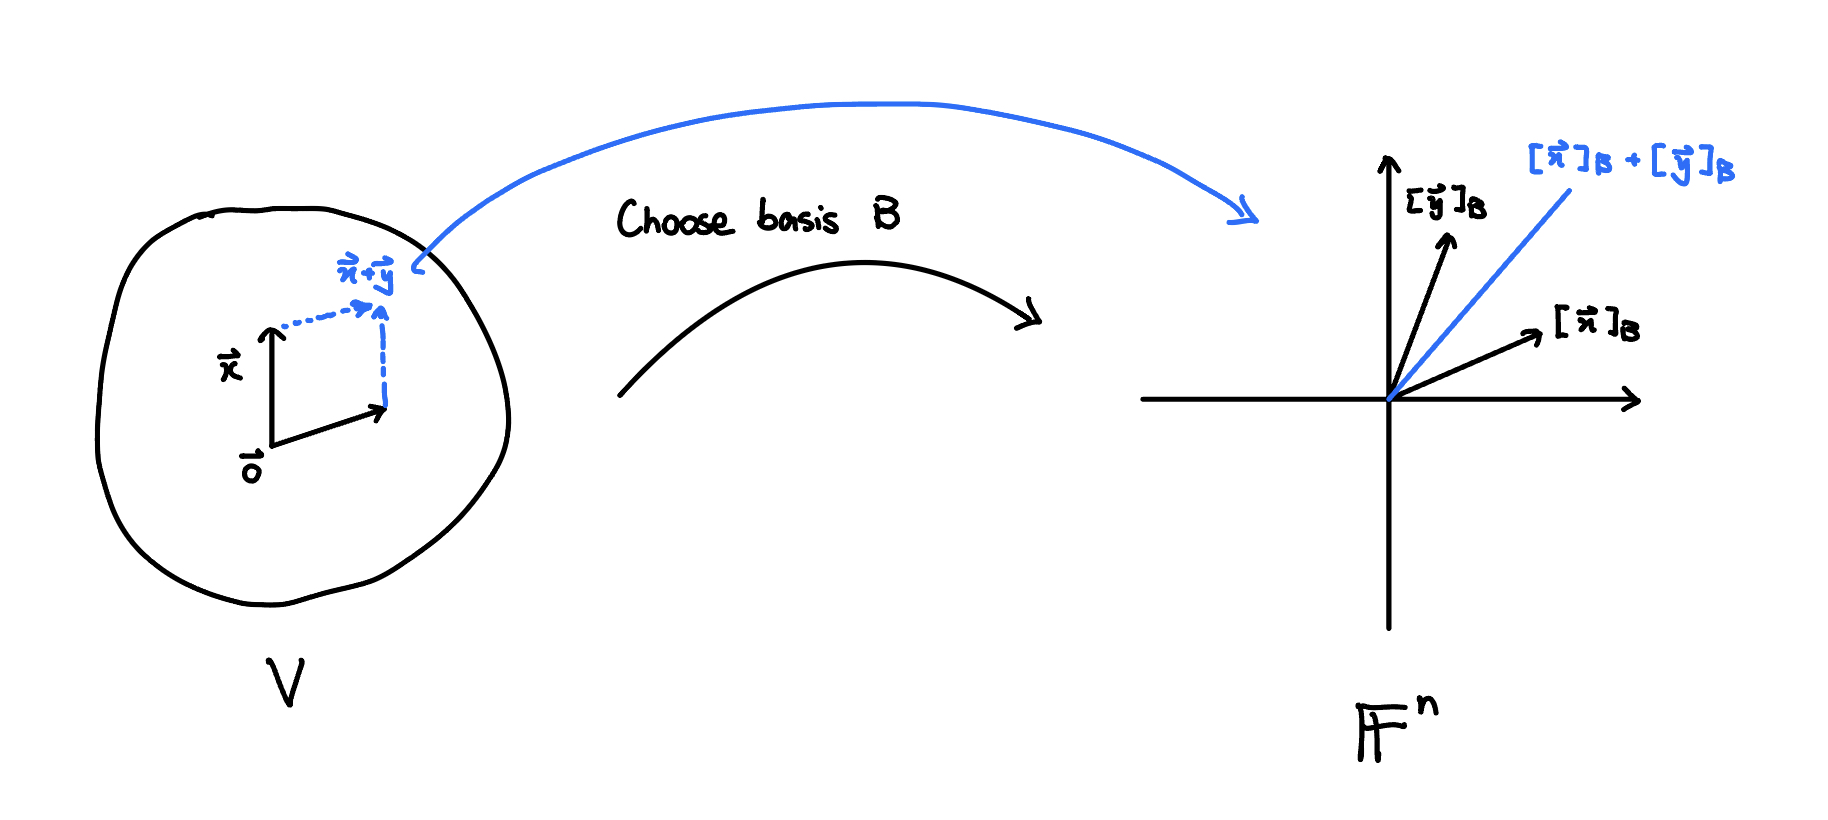
\includegraphics[scale=0.23]{img/vector_space--Fn.jpg}
    \caption{Translation between Abstract Vector Space and $\F^n$.}
\end{figure}


\begin{theorem}[\textbf{Linearity of Taking Coordinates}]
    \phantom{}\\
    Let $V$ be a finite-dimensional vector space over $\F$ with ordered basis $\mB$. Then
    \[[\vx + \vy]_{\mB} = [\vx]_{\mB} + [\vy]_{\mB} \quad \text{and} \quad [c\vx]_{\mB} = c[\vx]_{\mB}\]
    $\forall \vx,\vy \in V$ and all $c \in \F$.
\end{theorem}

\begin{proof}
    Exercise: prove addition.

    We will prove scalar multiplication. Suppose $\mB = \left\{ \vvb_1,\ldots,\vvb_n \right\}$. Suppose $\vx = a_1\vvb_1 + \cdots + a_n\vvb_n$.
    Then $\left[ \vx \right]_{\mB} = \cv{a_1 \\ \vdots \\ a_n}$. So $c\left[ \vx \right]_{\mB} = c\cv{a_1 \\ \vdots \\ a_n} = \cv{ca_1 \\ \vdots \\ ca_n}$.
    
    Now, $c\vx = c(a_1\vvb_1 + \cdots + a_n\vvb_n) = (ca_1)\vvb_1 + \cdots + (ca_n)\vvb_n$. Thus,
    \[\left[ c\vx \right]_{\mB} = \cv{ca_1 \\ \vdots \\ ca_n} = c\left[ \vx \right]_{\mB}.\]
\end{proof}






\newpage